% Fig. 3 -- model architecture (generic notation, top-to-bottom flow).
% Build:  pdflatex fig3_architecture.tex
% Sized for one IEEE column (~8.8 cm wide).
\documentclass[border=2pt]{standalone}
\usepackage{newtxtext,newtxmath}
\usepackage{tikz}
\usetikzlibrary{positioning,arrows.meta,calc,decorations.pathreplacing}

\definecolor{main}{RGB}{11,106,134}
\definecolor{tens}{RGB}{214,234,242}
\definecolor{stat}{RGB}{196,110,20}
\definecolor{opt}{RGB}{120,120,120}
\definecolor{outc}{RGB}{29,117,71}

\begin{document}
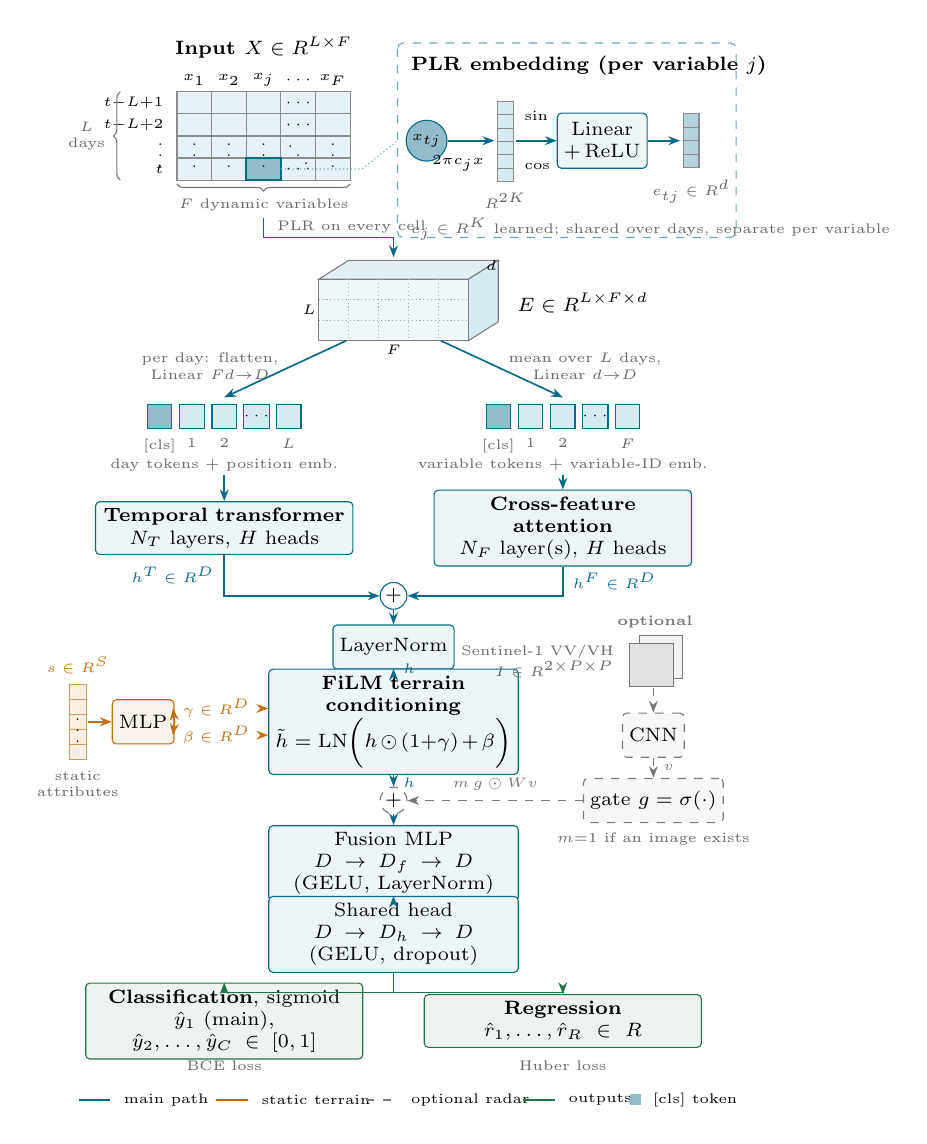
\begin{tikzpicture}[
  font=\scriptsize,
  box/.style={draw=main,fill=main!7,rounded corners=1.5pt,align=center,inner sep=2.4pt,minimum height=5.6mm},
  sbox/.style={box,draw=stat,fill=stat!8},
  obox/.style={box,draw=opt,fill=opt!6,dashed},
  gbox/.style={box,draw=outc,fill=outc!8},
  a/.style={-{Stealth[length=1.5mm]},semithick,main},
  sa/.style={a,stat},
  oa/.style={a,opt,dashed},
  ga/.style={a,outc},
  tok/.style={draw=main,fill=tens,minimum size=3.1mm,inner sep=0pt},
  cls/.style={tok,fill=main!45},
  note/.style={font=\tiny,text=black!60,align=center},
  brace/.style={decorate,decoration={brace,amplitude=2.5pt},thin,black!55}
]

%% ------------------------------------------------------------ 1. input matrix
\def\cw{0.44}\def\ch{0.28}
\def\gx{1.55}\def\gy{0}
\foreach \c in {0,...,4}{
  \foreach \r in {0,...,3}{
    \pgfmathsetmacro{\xa}{\gx+\c*\cw}\pgfmathsetmacro{\ya}{\gy-\r*\ch}
    \draw[black!45,fill=tens!60] (\xa,\ya) rectangle ++(\cw,-\ch);
  }}
% highlighted cell (row t, column j)
\fill[main!45] ({\gx+2*\cw},{\gy-3*\ch}) rectangle ++(\cw,-\ch);
\draw[main,thick] ({\gx+2*\cw},{\gy-3*\ch}) rectangle ++(\cw,-\ch);
% ellipsis column and row
\foreach \r in {0,1,3}{\node at ({\gx+3.5*\cw},{\gy-(\r+0.5)*\ch}) {\tiny$\cdots$};}
\foreach \c in {0,1,2,4}{\node at ({\gx+(\c+0.5)*\cw},{\gy-2.5*\ch}) {\tiny$\vdots$};}
\node at ({\gx+3.5*\cw},{\gy-2.5*\ch}) {\tiny$\ddots$};
% column / row labels
\foreach \c/\t in {0/{x_1},1/{x_2},2/{x_j},3/{\cdots},4/{x_F}}{
  \node[font=\tiny] at ({\gx+(\c+0.5)*\cw},{\gy+0.15}) {$\t$};}
\foreach \r/\t in {0/{t{-}L{+}1},1/{t{-}L{+}2},2/{\vdots},3/{t}}{
  \node[font=\tiny,anchor=east] at ({\gx-0.05},{\gy-(\r+0.5)*\ch}) {$\t$};}
\draw[brace] ({\gx-0.72},{\gy-4*\ch}) -- ({\gx-0.72},{\gy}) node[midway,left=2pt,note] {$L$\\days};
\draw[brace] ({\gx+5*\cw},{\gy-4*\ch-0.05}) -- ({\gx},{\gy-4*\ch-0.05}) node[midway,below=2pt,note] {$F$ dynamic variables};
\node[font=\scriptsize\bfseries,anchor=south] at ({\gx+2.5*\cw},{\gy+0.3}) {Input $X\in\mathbb{R}^{L\times F}$};

%% ------------------------------------------------------------ 2. PLR inset
\draw[main!60,dashed,rounded corners=2pt] (4.35,0.62) rectangle (8.65,-1.85);
\node[font=\scriptsize\bfseries,anchor=north west] at (4.4,0.58) {PLR embedding (per variable $j$)};
\node[draw=main,circle,fill=main!45,inner sep=1.2pt,font=\tiny] (x) at (4.72,-0.62) {$x_{tj}$};
% 2K vector
\foreach \k in {0,...,5}{\draw[black!45,fill=tens] (5.62,{-0.12-\k*0.17}) rectangle ++(0.2,-0.17);}
\node[font=\tiny,anchor=west] at (5.84,-0.3) {$\sin$};
\node[font=\tiny,anchor=west] at (5.84,-0.95) {$\cos$};
\node[note,anchor=north] at (5.72,-1.16) {$\mathbb{R}^{2K}$};
\draw[a] (x) -- (5.58,-0.62);
\node[font=\tiny,anchor=north] at (5.12,-0.68) {$2\pi c_j x$};
\node[box,minimum height=7mm] (lin) at (6.95,-0.62) {Linear\\+\,ReLU};
\draw[a] (5.86,-0.62) -- (lin);
% d vector
\foreach \k in {0,...,3}{\draw[black!45,fill=main!30] (7.98,{-0.28-\k*0.17}) rectangle ++(0.2,-0.17);}
\draw[a] (lin) -- (7.94,-0.62);
\node[note,anchor=north] at (8.08,-1.0) {$e_{tj}\in\mathbb{R}^{d}$};
\node[note,anchor=north west] at (4.4,-1.48) {$c_j\in\mathbb{R}^{K}$ learned; shared over days, separate per variable};
\draw[main!60,densely dotted] ({\gx+3*\cw},{\gy-3.5*\ch}) -- ({\gx+5*\cw+0.15},{\gy-3.5*\ch}) -- (4.35,-0.62);

%% ------------------------------------------------------------ 3. embedded tensor E
\def\tx{3.35}\def\ty{-2.38}\def\tw{1.9}\def\th{0.78}\def\dx{0.38}\def\dy{0.24}
\draw[black!50,fill=tens!70] (\tx,\ty) -- ++(\dx,\dy) -- ++(\tw,0) -- ++(-\dx,-\dy) -- cycle;
\draw[black!50,fill=tens] ({\tx+\tw},\ty) -- ++(\dx,\dy) -- ++(0,-\th) -- ++(-\dx,-\dy) -- cycle;
\draw[black!50,fill=tens!40] (\tx,\ty) rectangle ++(\tw,-\th);
\foreach \i in {1,...,4}{\draw[black!35,densely dotted] ({\tx+\i*\tw/5},\ty) -- ++(0,-\th);}
\foreach \i in {1,2}{\draw[black!35,densely dotted] (\tx,{\ty-\i*\th/3}) -- ++(\tw,0);}
\node[font=\tiny] at ({\tx-0.12},{\ty-\th/2}) {$L$};
\node[font=\tiny] at ({\tx+\tw/2},{\ty-\th-0.12}) {$F$};
\node[font=\tiny] at ({\tx+\tw+\dx/2+0.1},{\ty+\dy/2+0.05}) {$d$};
\node[font=\scriptsize,anchor=west] at ({\tx+\tw+\dx+0.12},{\ty-0.3}) {$E\in\mathbb{R}^{L\times F\times d}$};
\draw[a] ({\gx+2.5*\cw},{\gy-4*\ch-0.48}) -- ++(0,-0.25) -| ({\tx+\tw/2},{\ty+\dy+0.04});
\node[note,anchor=west] at ({\gx+2.5*\cw+0.05},{\gy-4*\ch-0.6}) {PLR on every cell};

%% ------------------------------------------------------------ 4. two branches
% --- temporal (left)
\def\lx{2.15}\def\rx{6.45}\def\ky{-4.12}
\node[cls] (lt0) at ({\lx-0.82},\ky) {};
\foreach \i/\t in {1/{},2/{},3/{\cdots},4/{}}{
  \node[tok] (lt\i) at ({\lx-0.82+\i*0.41},\ky) {\tiny$\t$};}
\node[note,anchor=north] at (lt0.south) {[cls]};
\node[note,anchor=north] at (lt1.south) {$1$};
\node[note,anchor=north] at (lt2.south) {$2$};
\node[note,anchor=north] at (lt4.south) {$L$};
\draw[a] ({\tx+0.35},{\ty-\th}) -- node[note,left=1pt,pos=0.45]{per day: flatten,\\Linear $Fd{\to}D$} ({\lx},{\ky+0.24});
\node[note] at ({\lx},{\ky-0.62}) {day tokens + position emb.};
\node[box,text width=3.1cm] (tenc) at ({\lx},{\ky-1.42}) {\textbf{Temporal transformer}\\$N_T$ layers, $H$ heads};
\draw[a] ({\lx},{\ky-0.74}) -- (tenc);
% --- feature (right)
\node[cls] (rt0) at ({\rx-0.82},\ky) {};
\foreach \i/\t in {1/{},2/{},3/{\cdots},4/{}}{
  \node[tok] (rt\i) at ({\rx-0.82+\i*0.41},\ky) {\tiny$\t$};}
\node[note,anchor=north] at (rt0.south) {[cls]};
\node[note,anchor=north] at (rt1.south) {$1$};
\node[note,anchor=north] at (rt2.south) {$2$};
\node[note,anchor=north] at (rt4.south) {$F$};
\draw[a] ({\tx+\tw-0.35},{\ty-\th}) -- node[note,right=1pt,pos=0.45]{mean over $L$ days,\\Linear $d{\to}D$} ({\rx},{\ky+0.24});
\node[note] at ({\rx},{\ky-0.62}) {variable tokens + variable-ID emb.};
\node[box,text width=3.1cm] (fenc) at ({\rx},{\ky-1.42}) {\textbf{Cross-feature attention}\\$N_F$ layer(s), $H$ heads};
\draw[a] ({\rx},{\ky-0.74}) -- (fenc);

%% ------------------------------------------------------------ 5. merge
\begin{scope}[yshift=-0.45cm]
\node[draw=main,circle,inner sep=0.6pt,fill=white,font=\scriptsize] (plus1) at (4.3,-5.95) {$+$};
\draw[a] (tenc.south) |- node[pos=0.25,left,font=\tiny]{$h^{T}\in\mathbb{R}^{D}$} (plus1.west);
\draw[a] (fenc.south) |- node[pos=0.25,right,font=\tiny]{$h^{F}\in\mathbb{R}^{D}$} (plus1.east);
\node[box] (ln) at (4.3,-6.6) {LayerNorm};
\draw[a] (plus1) -- (ln);

%% ------------------------------------------------------------ 6. FiLM
\node[box,text width=3.0cm] (film) at (4.3,-7.55) {\textbf{FiLM terrain conditioning}\\$\tilde h=\mathrm{LN}\big(h\odot(1{+}\gamma)+\beta\big)$};
\draw[a] (ln) -- node[right,font=\tiny]{$h$} (film);
% static vector
\foreach \k in {0,...,4}{\draw[stat!70,fill=stat!12] (0.18,{-7.08-\k*0.19}) rectangle ++(0.22,-0.19);}
\node[font=\tiny] at (0.29,-7.555) {$\vdots$};
\node[font=\tiny,text=stat,anchor=south] at (0.29,-7.06) {$s\in\mathbb{R}^{S}$};
\node[note,anchor=north] at (0.29,-8.05) {static\\attributes};
\node[sbox] (mlp) at (1.12,-7.55) {MLP};
\draw[sa] (0.42,-7.55) -- (mlp);
\node[font=\tiny,text=stat] (gam) at (2.05,-7.38) {$\gamma\in\mathbb{R}^{D}$};
\node[font=\tiny,text=stat] (bet) at (2.05,-7.72) {$\beta\in\mathbb{R}^{D}$};
\draw[sa] (mlp.east) -- (gam.west);
\draw[sa] (mlp.east) -- (bet.west);
\draw[sa] (gam.east) -- (film.west|-gam);
\draw[sa] (bet.east) -- (film.west|-bet);

%% ------------------------------------------------------------ 7. optional radar branch
\node[font=\tiny\bfseries,text=opt] at (7.62,-6.28) {optional};
\draw[opt,fill=opt!10] (7.42,-6.45) rectangle ++(0.55,-0.55);
\draw[opt,fill=opt!22] (7.30,-6.55) rectangle ++(0.55,-0.55);
\node[note,anchor=east,align=right] at (7.22,-6.78) {Sentinel-1 VV/VH\\$I\in\mathbb{R}^{2\times P\times P}$};
\node[obox] (cnn) at (7.6,-7.72) {CNN};
\draw[oa] (7.6,-7.12) -- (cnn);
\node[obox] (gate) at (7.6,-8.55) {gate $g=\sigma(\cdot)$};
\draw[oa] (cnn) -- node[right,font=\tiny]{$v$} (gate);
\node[draw=opt,dashed,circle,inner sep=0.6pt,fill=white,font=\scriptsize] (plus2) at (4.3,-8.55) {$+$};
\draw[a] (film) -- node[right,font=\tiny]{$\tilde h$} (plus2);
\draw[oa] (gate) -- node[above,font=\tiny]{$m\,g\odot Wv$} (plus2);
\node[note,anchor=north] at (gate.south) {$m{=}1$ if an image exists};

%% ------------------------------------------------------------ 8. fusion + head
\node[box,text width=3.0cm] (fuse) at (4.3,-9.35) {Fusion MLP $D\to D_f\to D$\\(GELU, LayerNorm)};
\draw[a] (plus2) -- (fuse);
\node[box,text width=3.0cm] (head) at (4.3,-10.25) {Shared head $D\to D_h\to D$\\(GELU, dropout)};
\draw[a] (fuse) -- (head);

%% ------------------------------------------------------------ 9. outputs
\node[gbox,text width=3.35cm] (cls) at (2.15,-11.35) {\textbf{Classification}, sigmoid\\$\hat y_1$ (main), $\hat y_2,\dots,\hat y_C\in[0,1]$};
\node[gbox,text width=3.35cm] (reg) at (6.45,-11.35) {\textbf{Regression}\\$\hat r_1,\dots,\hat r_R\in\mathbb{R}$};
\draw[ga] (head.south) -- ++(0,-0.25) -| (cls.north);
\draw[ga] (head.south) -- ++(0,-0.25) -| (reg.north);
\node[note] at (2.15,-11.92) {BCE loss};
\node[note] at (6.45,-11.92) {Huber loss};

%% ------------------------------------------------------------ legend
\begin{scope}[shift={(0.3,-12.35)},font=\tiny]
  \draw[main,semithick] (0,0) -- (0.4,0); \node[anchor=west] at (0.45,0) {main path};
  \draw[stat,semithick] (1.75,0) -- (2.15,0); \node[anchor=west] at (2.2,0) {static terrain};
  \draw[opt,semithick,dashed] (3.65,0) -- (4.05,0); \node[anchor=west] at (4.1,0) {optional radar};
  \draw[outc,semithick] (5.65,0) -- (6.05,0); \node[anchor=west] at (6.1,0) {outputs};
  \fill[main!45] (7.0,-0.07) rectangle ++(0.14,0.14); \node[anchor=west] at (7.17,0) {[cls] token};
\end{scope}
\end{scope}
\end{tikzpicture}
\end{document}
